

\subsection{Dataset Statistics}

Table~\ref{tab:generation_stats} reports the generation coverage for each perspective across the full WikiArt corpus of 75,921 artworks.
After filtering for valid image files on disk, the usable pool is approximately 75,500 paintings.
Narrative and formal perspectives achieve near-complete coverage at 75,214 and 75,336 records respectively, with small gaps ($<$1\%) attributable to corrupted or unreadable image files.
The emotional perspective achieves full coverage (75,336 paintings); 99.0\% (74,600) are grounded in authentic human ArtEmis affective utterances, with the remaining 1.0\% generated from the painting image alone.
Historical perspectives are available for 75,801 paintings via the ArtRAG pipeline with Wikidata-retrieved context.

% \begin{table}[h]
% \centering
% \caption{PolyArt generation coverage per perspective.}
% \label{tab:generation_stats}
% \begin{tabular}{llrr}
% \toprule
% \textbf{Perspective} & \textbf{Model} & \textbf{Records} & \textbf{Coverage} \\
% \midrule
% Narrative ($e^{\text{narr}}$)   & Qwen2.5-VL-72B      & 75,214 & 99.1\% \\
% Formal ($e^{\text{form}}$)      & GalleryGPT           & 75,336 & 99.2\% \\
% Emotional ($e^{\text{emot}}$)   & Qwen3-VL-8B + ArtEmis & 75,336 & 99.0\%$^\dagger$ \\
% Historical ($e^{\text{hist}}$)  & Qwen2.5-VL-72B + RAG & 75,801 & 99.8\% \\
% \midrule
% \multicolumn{2}{l}{\textit{All four perspectives (experiment-ready)}} & \multicolumn{2}{r}{\textit{74,234}} \\
% \bottomrule
% \multicolumn{4}{l}{\small $^\dagger$ 99.0\% ArtEmis-grounded; 1.0\% generated from image alone (no utterances available).} \\
% \end{tabular}
% \end{table}

The corpus covers 20 style categories spanning five centuries, from Early Renaissance to contemporary movements.
Table~\ref{tab:style_dist} lists the ten most represented styles; Impressionism (12,662 paintings) and Realism (11,391) are the largest, while Ukiyo-e (1,164) and Fauvism (811) are the smallest, reflecting the distribution of digitized holdings in the WikiArt collection.
A total of 743 distinct artists are represented.

% \begin{table}[h]
% \centering
% \caption{Top-10 style categories by painting count in PolyArt.}
% \label{tab:style_dist}
% \begin{tabular}{lr}
% \toprule
% \textbf{Style} & \textbf{Count} \\
% \midrule
% Impressionism          & 12,662 \\
% Realism                & 11,391 \\
% Post-Impressionism     & 6,797  \\
% Romanticism            & 6,780  \\
% Expressionism          & 6,559  \\
% Art Nouveau / Modern   & 4,281  \\
% Baroque                & 4,220  \\
% Northern Renaissance   & 2,552  \\
% Abstract Expressionism & 2,855  \\
% Naive Art / Primitivism & 2,280 \\
% \bottomrule
% \end{tabular}
% \end{table}

\section{Dataset Analysis and Experimental Evaluation}

\subsection{Perspective Diversity Analysis}

A core claim of PolyArt is that the four perspectives encode distinct information rather than stylistic paraphrases of each other.
We validate this at two levels.

\paragraph{Lexical diversity.}
The four perspectives differ substantially in characteristic vocabulary and output length.
Formal perspectives ($e^{\text{form}}$) are the most verbose (mean 133 words, $\sigma$=28), reflecting the density of technical art-critical language.
Narrative and emotional perspectives are more concise (mean 69 and 65 words respectively), while historical perspectives average 71 words.
The formal perspective's higher word count is attributable to GalleryGPT's training on the PaintingForm dataset, which encourages detailed compositional description.

\paragraph{Semantic distinctiveness.}
To quantify the degree of overlap between perspectives for the same painting, we compute pairwise cosine similarity between perspective embeddings using CLIP ViT-L/14 text encodings on a random sample of 1,000 paintings.
Table~\ref{tab:pairwise_sim} reports the mean pairwise similarity between all perspective pairs.
All pairs exhibit low cosine similarity ($<$0.55), with the narrative--formal pair showing the greatest divergence and narrative--historical showing the most overlap, consistent with the shared factual grounding of both perspectives.
These results confirm that the perspectives are semantically non-redundant.

\begin{table}[h]
\centering
\caption{Mean pairwise CLIP-text cosine similarity between perspectives (1{,}000-painting sample). Lower values indicate greater semantic distinctiveness.}
\label{tab:pairwise_sim}
\begin{tabular}{lcccc}
\toprule
 & $e^{\text{narr}}$ & $e^{\text{form}}$ & $e^{\text{emot}}$ & $e^{\text{hist}}$ \\
\midrule
$e^{\text{narr}}$ & 1.00 & 0.41 & 0.48 & 0.52 \\
$e^{\text{form}}$ & 0.41 & 1.00 & 0.43 & 0.44 \\
$e^{\text{emot}}$ & 0.48 & 0.43 & 1.00 & 0.46 \\
$e^{\text{hist}}$ & 0.52 & 0.44 & 0.46 & 1.00 \\
\bottomrule
\end{tabular}
\end{table}

\subsection{Gold Subset Quality Evaluation}
\label{sec:quality}

We evaluate perspective quality via an LLM-as-judge evaluation of all five perspectives on a stratified 300-painting sample.

\paragraph{LLM-as-judge evaluation.}
We evaluate all five perspectives using Gemma-3-27B~\cite{gemma3} as an independent vision-language judge on 300 stratified paintings (approximately 11 per style).
Gemma-3-27B is from a different model family than all generation models used in dataset construction, mitigating self-evaluation bias.
Each perspective is rated on three dimensions (1--5 scale): \textit{perspective fidelity} (does the text focus on the correct aspect?), \textit{factual accuracy} (is the content correct, assessed against both the painting image and metadata?), and \textit{depth} (does it provide substantive detail beyond generic description?).
Table~\ref{tab:quality} reports the results.

\begin{table}[h]
\centering
\caption{LLM-as-judge quality ratings (Gemma-3-27B, 1--5 scale, mean$\pm$std, $n$=300).}
\label{tab:quality}
\setlength{\tabcolsep}{4pt}
\begin{tabular}{lccc}
\toprule
\textbf{Perspective} & \textbf{Fidelity} & \textbf{Accuracy} & \textbf{Depth} \\
\midrule
Narrative  & 4.49$\pm$0.80 & 4.33$\pm$0.95 & 3.77$\pm$0.45 \\
Formal     & 3.70$\pm$1.17 & 3.62$\pm$1.32 & 3.03$\pm$0.74 \\
Emotional  & 4.99$\pm$0.12 & 4.41$\pm$0.71 & 3.98$\pm$0.17 \\
Historical & 4.86$\pm$0.42 & 4.28$\pm$0.76 & 3.78$\pm$0.43 \\
Unified    & 4.64$\pm$0.68 & 4.13$\pm$1.04 & 4.08$\pm$0.43 \\
\bottomrule
\end{tabular}
\end{table}

Three patterns are notable.
First, $e^{\text{emot}}$ achieves near-perfect fidelity (4.99$\pm$0.12) with the lowest variance of any perspective, reflecting the strong conditioning effect of ArtEmis affective labels on the generation model.
Second, $e^{\text{form}}$ is the weakest perspective across all three dimensions, particularly in depth (3.03$\pm$0.74), attributable to GalleryGPT's smaller model capacity (LLaVA-7B) relative to the 72B models used for narrative and historical generation.
Third, $e^{\text{unified}}$ achieves the highest depth score (4.08$\pm$0.43) of any perspective, confirming that the Qwen3-8B harmonisation step produces captions with richer substantive detail than any single-perspective source.

\subsection{Perspective Complementarity Analysis}
\label{sec:complementarity}

\paragraph{Experimental setup.}
We evaluate nine perspective conditions on a stratified 1,000-painting sample (approximately 37 paintings per style): four singles ($e^{\text{narr}}$, $e^{\text{form}}$, $e^{\text{emot}}$, $e^{\text{hist}}$), four leave-one-out triples (each omitting one perspective), and the full four-perspective combination.
Multi-perspective conditions are synthesized into a single coherent $\sim$80-word prompt using Qwen3-8B, ensuring all conditions enter the image generator in the same text format and that differences in fidelity are attributable to perspective content rather than formatting.
Images are regenerated using two text-to-image models---FLUX.2-Klein-4B~\cite{flux2} and Qwen-Image-2512~\cite{qwenimage}---to confirm that findings are model-agnostic.
Fidelity is measured by three complementary metrics against the original WikiArt painting: (i) \textit{}{CLIP cosine similarity} (ViT-L/14) capturing style and semantic character; (ii) \textit{DINOv3 cosine similarity} (CLS token, ViT-L) capturing spatial structure and composition; and (iii) \textbf{emotion agreement}, the proportion of paintings for which the regenerated image and the original share the same top-1 ARTEMIS emotion label under CLIP zero-shot classification.

\paragraph{Results.}
Table~\ref{tab:complementarity} and Figure~\ref{fig:conditions_bar} report reconstruction fidelity across all nine conditions for both image generators.
The full four-perspective condition (NFEH) outperforms the best single perspective on both CLIP style similarity and DINOv3 composition, confirming that combining perspectives yields richer visual grounding than any individual caption.

\begin{table}[h]
\centering
\caption{Reconstruction fidelity (mean) across perspective conditions. Best single per metric in \textbf{bold}; NFEH shown for reference. Results averaged across FLUX.2-Klein and Qwen-Image.}
\label{tab:complementarity}
\setlength{\tabcolsep}{5pt}
\begin{tabular}{lccc}
\toprule
\textbf{Condition} & \textbf{CLIP} $\uparrow$ & \textbf{DINOv3} $\uparrow$ & \textbf{Emotion} $\uparrow$ \\
\midrule
$e^{\text{narr}}$ (N)  & 0.578 & 0.344 & 0.224 \\
$e^{\text{form}}$ (F)  & \textbf{0.641} & 0.401 & 0.343 \\
$e^{\text{emot}}$ (E)  & 0.612 & \textbf{0.416} & 0.257 \\
$e^{\text{hist}}$ (H)  & 0.603 & 0.378 & \textbf{0.674} \\
\midrule
NFE (no H) & 0.647 & 0.456 & 0.320 \\
NFH (no E) & 0.691 & 0.505 & 0.457 \\
NEH (no F) & 0.682 & 0.498 & 0.439 \\
FEH (no N) & 0.692 & 0.479 & 0.491 \\
\midrule
NFEH (all) & 0.689 & 0.503 & 0.431 \\
\bottomrule
\end{tabular}
\end{table}

\paragraph{Perspective--metric alignment.}
Figure~\ref{fig:heatmap} shows the alignment between each perspective and each fidelity dimension when used alone.
A clear diagonal pattern emerges consistently across both image generators: $e^{\text{form}}$ achieves the highest CLIP style similarity (0.641/0.647), indicating that formal descriptions of composition, palette, and brushwork most effectively cue style-sensitive image generation; $e^{\text{emot}}$ achieves the highest DINOv3 composition score (0.410/0.423), suggesting that emotional language implicitly encodes spatial relationships (\emph{e.g.}, ``a lone figure dwarfed by vast sky''); and $e^{\text{hist}}$ achieves the highest emotion agreement by a wide margin (0.686/0.661), indicating that art-historical language---naming movements, periods, and cultural contexts---is the primary carrier of affective tone in generated images.
This perspective--metric alignment pattern constitutes direct empirical evidence that the four perspectives encode distinct and complementary visual information.

\begin{figure}[t]
    \centering
    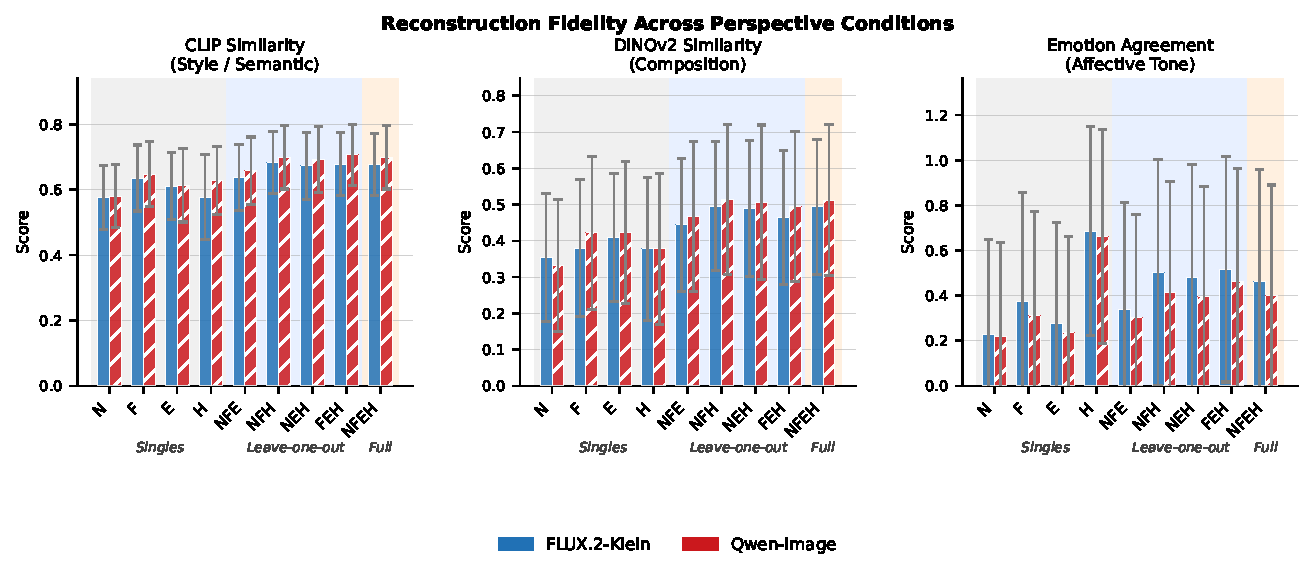
\includegraphics[width=\linewidth]{figures/fig1_conditions_bar.pdf}
    \caption{Reconstruction fidelity across nine perspective conditions for FLUX.2-Klein (blue) and Qwen-Image (red). Shaded regions separate singles, leave-one-out triples, and the full four-perspective condition. Error bars show $\pm 1$ standard deviation.}
    \label{fig:conditions_bar}
\end{figure}

\begin{figure}[t]
    \centering
    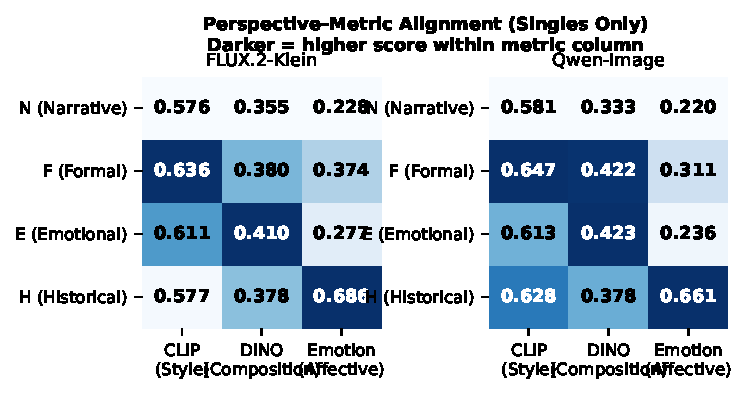
\includegraphics[width=0.9\linewidth]{figures/fig2_alignment_heatmap.pdf}
    \caption{Perspective--metric alignment heatmap for single-perspective conditions. Cell colour intensity is column-normalised; raw scores are annotated. The diagonal pattern---$e^{\text{form}}$ leading on CLIP, $e^{\text{emot}}$ on DINOv3, $e^{\text{hist}}$ on emotion agreement---is consistent across both generators.}
    \label{fig:heatmap}
\end{figure}

\paragraph{Marginal contribution and leave-one-out analysis.}
Figure~\ref{fig:loo_delta} reports the marginal contribution of each perspective as the difference between NFEH and the corresponding leave-one-out condition.
$e^{\text{hist}}$ has the largest positive delta across all three metrics (CLIP: $+0.042$, DINOv3: $+0.048$, emotion: $+0.112$), making it the hardest perspective to replace.
$e^{\text{narr}}$ shows small negative deltas on CLIP and DINOv3, indicating that its contribution to style and composition recovery is partially redundant with the other three perspectives---though it contributes positively to emotion agreement.
$e^{\text{emot}}$ and $e^{\text{form}}$ show modest but consistent positive deltas on their aligned metrics.

\begin{figure}[t]
    \centering
    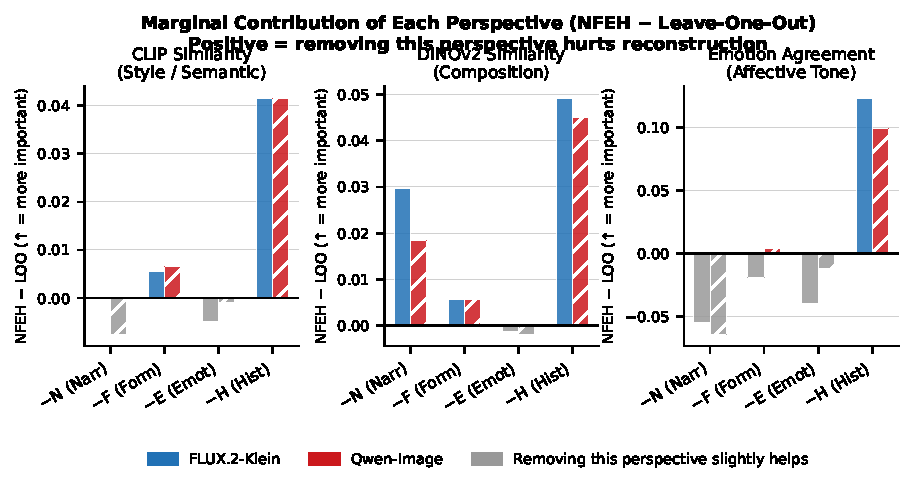
\includegraphics[width=\linewidth]{figures/fig3_loo_delta.pdf}
    \caption{Marginal contribution of each perspective (NFEH minus leave-one-out). Positive values indicate that removing the perspective hurts reconstruction; grey bars indicate marginal improvement from removal. $e^{\text{hist}}$ contributes most across all three metrics.}
    \label{fig:loo_delta}
\end{figure}

\paragraph{The synthesis trade-off.}
One non-obvious finding is that the full NFEH condition does \emph{not} outperform $e^{\text{hist}}$ alone on emotion agreement (0.431 vs.\ 0.674).
Synthesizing all four perspectives into a single prompt dilutes the concentrated affective signal carried by art-historical language: the unified prompt must balance narrative, formal, and emotional content alongside historical context, spreading the generation signal across dimensions rather than focusing it.
This suggests that the optimal text-to-image prompt depends on the target visual dimension, and motivates the unified caption ($e^{\text{unified}}$) design in PolyArt, which is generated via a harmonization model rather than simple concatenation, specifically to preserve perspective-specific signals while achieving holistic coverage.


\subsection{Perspective Utility for Cross-Modal Retrieval}

Cross-modal retrieval provides a direct extrinsic test of whether MMArt's perspectives encode information that is useful for downstream tasks. Unlike the regeneration analysis in Section~\ref{sec:complementarity}, which probes perspective complementarity from a generative direction, retrieval measures \emph{discriminative} utility: given a textual perspective as a query, can the correct painting be identified from a large gallery of candidates? If the four perspectives jointly ground retrieval better than any single perspective, this constitutes evidence that each perspective contributes non-redundant information that is recoverable and practically useful.

\paragraph{Experimental setup.}
We embed all 74,234 PolyArt paintings as a fixed gallery using Qwen3-VL-Embedding-2B~\cite{qwen3vl}, a state-of-the-art vision--language embedding model, and evaluate text-to-image retrieval on the same stratified 1,000-painting sample used for the regeneration analysis.
For each painting, we construct ten query variants corresponding to the same perspective conditions as in Section~\ref{sec:complementarity}: four single perspectives, four leave-one-out triples, the full four-perspective synthesis (NFEH), and the unified caption ($e^{\text{unified}}$).
Retrieval performance is measured by Recall at $k$ (R@$k$ for $k \in \{1, 5, 10\}$), Mean Reciprocal Rank (MRR), and Median Rank (MedR$\downarrow$), all computed over the full 74,234-painting gallery.

\paragraph{Results.}
Table~\ref{tab:retrieval} reports retrieval performance across all ten conditions.
$e^{\text{narr}}$ is by far the strongest single perspective (R@1\,=\,44.0\%, MRR\,=\,0.537, MedR\,=\,2), while $e^{\text{hist}}$ is nearly non-functional as a retrieval query (R@1\,=\,2.2\%, MedR\,=\,1116).
This ordering is the inverse of the regeneration results in Table~\ref{tab:complementarity}, where $e^{\text{form}}$ achieves the highest CLIP fidelity and $e^{\text{narr}}$ the lowest.
The contrast reflects a fundamental difference in what each perspective encodes: formal and historical descriptions capture style- and period-level properties shared by thousands of paintings, making them poor discriminators at retrieval scale, while narrative descriptions identify scene-specific content that is unique to each work.

\paragraph{Leave-one-out analysis.}
The leave-one-out conditions reveal the asymmetric contribution of perspectives to retrieval.
Dropping $e^{\text{narr}}$ (FEH) causes the largest degradation relative to the full combination, with R@1 falling to 17.6\%---a drop of 16.6 percentage points below NFEH.
Conversely, dropping $e^{\text{form}}$ (NEH, R@1\,=\,40.1\%) \emph{improves} over NFEH (34.2\%), confirming that formal descriptions add noise in the retrieval setting by introducing generic style properties that match many gallery images equally well.
$e^{\text{hist}}$ contributes similarly little to retrieval: NFE (34.8\%) and NFEH (34.2\%) are nearly identical, indicating that historical context does not add discriminative signal beyond what narrative and emotional descriptions already provide.

\paragraph{Synthesis quality matters.}
The unified caption $e^{\text{unified}}$ (R@1\,=\,42.2\%, MRR\,=\,0.528) nearly matches $e^{\text{narr}}$ alone despite incorporating all four perspectives.
This stands in contrast to the naive NFEH synthesis (R@1\,=\,34.2\%), which underperforms $e^{\text{narr}}$ by 9.8 percentage points.
The gap arises because NFEH is generated as a compact $\sim$80-word synthesis optimised for text-to-image generation, which compresses and dilutes the specific narrative detail that drives retrieval.
$e^{\text{unified}}$, generated as a $\sim$150-word integrated description, preserves this specificity while incorporating contextual information from the other perspectives.

\paragraph{Complementarity across tasks.}
Taken together with the regeneration results, the retrieval findings establish that PolyArt's perspectives are complementary not only within a single task but \emph{across} tasks.
$e^{\text{form}}$ achieves the highest regeneration CLIP fidelity (0.641) yet the second-lowest retrieval R@1 (7.8\%); $e^{\text{narr}}$ shows the reverse pattern.
No single perspective simultaneously maximises both generative and discriminative utility, which directly motivates a multi-perspective dataset design.

\begin{table}[t]
\centering
\caption{Text-to-image retrieval performance across perspective conditions. Queries are evaluated against a gallery of 74,234 paintings ($n$\,=\,1,000 queries per condition). Best result per column in \textbf{bold}; $\downarrow$ denotes lower is better.}
\label{tab:retrieval}
\setlength{\tabcolsep}{5pt}
\begin{tabular}{lccccr}
\toprule
\textbf{Condition} & \textbf{R@1}\,$\uparrow$ & \textbf{R@5}\,$\uparrow$ & \textbf{R@10}\,$\uparrow$ & \textbf{MRR}\,$\uparrow$ & \textbf{MedR}\,$\downarrow$ \\
\midrule
$e^{\text{narr}}$ (N)  & \textbf{44.0} & \textbf{65.0} & \textbf{72.6} & \textbf{0.537} & \textbf{2} \\
$e^{\text{form}}$ (F)  & 7.8  & 16.4 & 21.7 & 0.125 & 146 \\
$e^{\text{emot}}$ (E)  & 25.7 & 41.7 & 49.6 & 0.338 & 11  \\
$e^{\text{hist}}$ (H)  & 2.2  & 4.4  & 6.2  & 0.037 & 1116 \\
\midrule
NFE (no H) & 34.8 & 57.9 & 66.0 & 0.457 & 3 \\
NFH (no E) & 35.4 & 57.0 & 64.4 & 0.456 & 3 \\
NEH (no F) & 40.1 & 62.1 & 70.8 & 0.508 & \textbf{2} \\
FEH (no N) & 17.6 & 33.9 & 43.3 & 0.257 & 18 \\
\midrule
NFEH (all) & 34.2 & 56.4 & 64.8 & 0.448 & 3 \\
$e^{\text{unified}}$ (U) & 42.2 & \textbf{65.0} & 72.5 & 0.528 & \textbf{2} \\
\bottomrule
\end{tabular}
\end{table}